\documentclass[11pt]{article}
\usepackage[letterpaper,margin=0.9in]{geometry}
\usepackage[T1]{fontenc}
\usepackage{lmodern}
\usepackage{microtype}
\usepackage{xcolor}
\usepackage{graphicx}
\usepackage{array,tabularx,booktabs}
\usepackage{enumitem}
\usepackage{caption}
\usepackage[hidelinks]{hyperref}

\setlength{\parindent}{0pt}
\setlength{\parskip}{5pt}
\setlist[itemize]{leftmargin=1.3em,topsep=2pt,itemsep=2pt,parsep=0pt}
\setlist[enumerate]{leftmargin=1.5em,topsep=2pt,itemsep=2pt,parsep=0pt}
\captionsetup{font=small,labelfont=bf,skip=4pt}
\newcolumntype{Y}{>{\raggedright\arraybackslash}X}
\definecolor{accent}{HTML}{C2571A}
\definecolor{boxbg}{HTML}{F6F1EC}
\newcommand{\keybox}[1]{\par\smallskip\noindent\colorbox{boxbg}{\parbox{\dimexpr\linewidth-2\fboxsep}{\vspace{3pt}#1\vspace{3pt}}}\par\smallskip}

\title{\textbf{Benchmark Cartography, explained}\\[2pt]
\large Finding mistakes in an AI exam's answer key, for readers new to the topic}
\author{Team 21: Arman Samayam and Padmapriya Venkatesh\\
\small DS-GA 3001 Visualization for Machine Learning, NYU, Fall 2026}
\date{}

\begin{document}
\maketitle
\vspace{-2em}

\keybox{\textbf{In one sentence.} By having 150 AI models ``vote'' on every exam question, we can
spot questions whose official answer is probably wrong, often suggest the right one, and show in an
interactive tool that these mistakes do reshuffle the middle of the AI leaderboard, though not the
top. Because the models can sometimes all be wrong together, a human still makes the final call.}

\section{Background: how AI models get graded}

Companies and researchers build \textbf{AI language models}, the kind of system behind ChatGPT. To
compare them, everyone gives the models the same \textbf{exam}, called a \textbf{benchmark}.

One of the most famous is \textbf{MMLU}:
\begin{itemize}
  \item about \textbf{14,000 multiple-choice questions}, each with four options (A, B, C, D);
  \item spread over \textbf{57 subjects}, such as biology, history, law, math, psychology and virology;
  \item every question comes with an \textbf{answer key}: the ``official'' correct letter.
\end{itemize}
A model's score is simply the percentage it gets right. Public websites called
\textbf{leaderboards} rank hundreds of models by that score, like a league table, and people use
these rankings to decide which model is ``better''.

\section{The problem: the answer key has mistakes}

Imagine a school exam where the teacher's answer sheet has a few wrong answers. A student who picks
the truly correct answer gets marked \emph{wrong}. That is unfair, and it can change who comes top of
the class.

This happens with MMLU. A research team (\textbf{MMLU-Redux}) had experts check 5,700 of the 14,000
questions by hand. They found:
\begin{itemize}
  \item about \textbf{2\%} have a \textbf{wrong answer key}: the official answer is simply incorrect;
  \item about \textbf{4--5\%} more are flawed in other ways: unclear wording, more than one right
    answer, or no right answer.
\end{itemize}
Two facts make this matter:
\begin{itemize}
  \item \textbf{About 8,300 questions have never been checked.} There are surely more mistakes there.
  \item \textbf{Models on leaderboards are separated by tiny margins}, often less than a fifth of a
    percentage point between neighbours. A handful of bad questions could swap their positions.
\end{itemize}
So the project asks two practical questions:
\begin{enumerate}
  \item Can we \textbf{find} the broken questions automatically, including the unchecked ones?
  \item Does fixing them \textbf{actually change the leaderboard}?
\end{enumerate}

\section{The core idea: let 150 AI models ``vote''}

Checking 14,000 questions by hand is too slow. But a public archive (the \textbf{Open LLM
Leaderboard}) already stores \textbf{how hundreds of models answered every question}. We collected
\textbf{150 models}, all tested in exactly the same way so the comparison is fair.

The intuition, in school terms:
\begin{itemize}
  \item \textbf{A hard but fair question:} weak students get it wrong; strong students get it right.
  \item \textbf{A question with a wrong key:} even the \textbf{best students} get it ``wrong'', and they
    \textbf{all pick the same other answer}. That shared answer is usually the real correct one.
\end{itemize}
So if the strongest models all agree on an answer different from the key, that is a red flag that
the \emph{key} is wrong, not the models.

The idea is adapted from an earlier technique called \textbf{Dataset Cartography}
(``cartography'' means map-making), which finds mislabelled data by watching \emph{one} model learn
over time. We swapped ``one model over time'' for ``\textbf{many models at once}''. Hence the name.

\section{What we measure for every question}

For every question and every model we know how much the model ``believed'' each of A, B, C and D (a
probability). From those numbers we compute a few simple scores:

\begin{center}\small
\begin{tabularx}{\linewidth}{@{}p{3.2cm}YY@{}}
\toprule
\textbf{Score} & \textbf{Plain meaning} & \textbf{What it suggests} \\
\midrule
Confidence & On average, how much models believed the official answer & Low: models reject the key \\
Variability & How much models disagree with each other & Low: models agree, even if \emph{against} the key \\
Top-tier confidence & Confidence among only the \textbf{30 strongest models} & The best warning sign \\
Consensus alternative & The answer the strongest models pick instead & Often the real answer, so it \textbf{suggests a fix} \\
Consensus share & What fraction of the top 30 picked that alternative & 100\%: unanimous; 45\%: split \\
Ability alignment & Do stronger models do \emph{better} on this question? & If they do \emph{worse}, something is off \\
\bottomrule
\end{tabularx}
\end{center}

\textbf{The standard comparison: IRT.} \textbf{Item Response Theory} is an established statistical
method from exam design. For each question it estimates a \textbf{difficulty} (how hard it is) and a
\textbf{discrimination} (does it separate strong test-takers from weak ones?). A question where
strong test-takers do \emph{worse} has negative discrimination, a classic sign of a bad key. Our
instructor asked us to show \textbf{what our approach adds beyond IRT}, so IRT is our main comparison
throughout.

\section{What we built: an interactive visual tool}

The main deliverable is a website built with the visualization library \textbf{D3}:\\
\url{https://armansam17.github.io/Benchmark-Cartography/}

\begin{figure}[!htb]
  \centering
  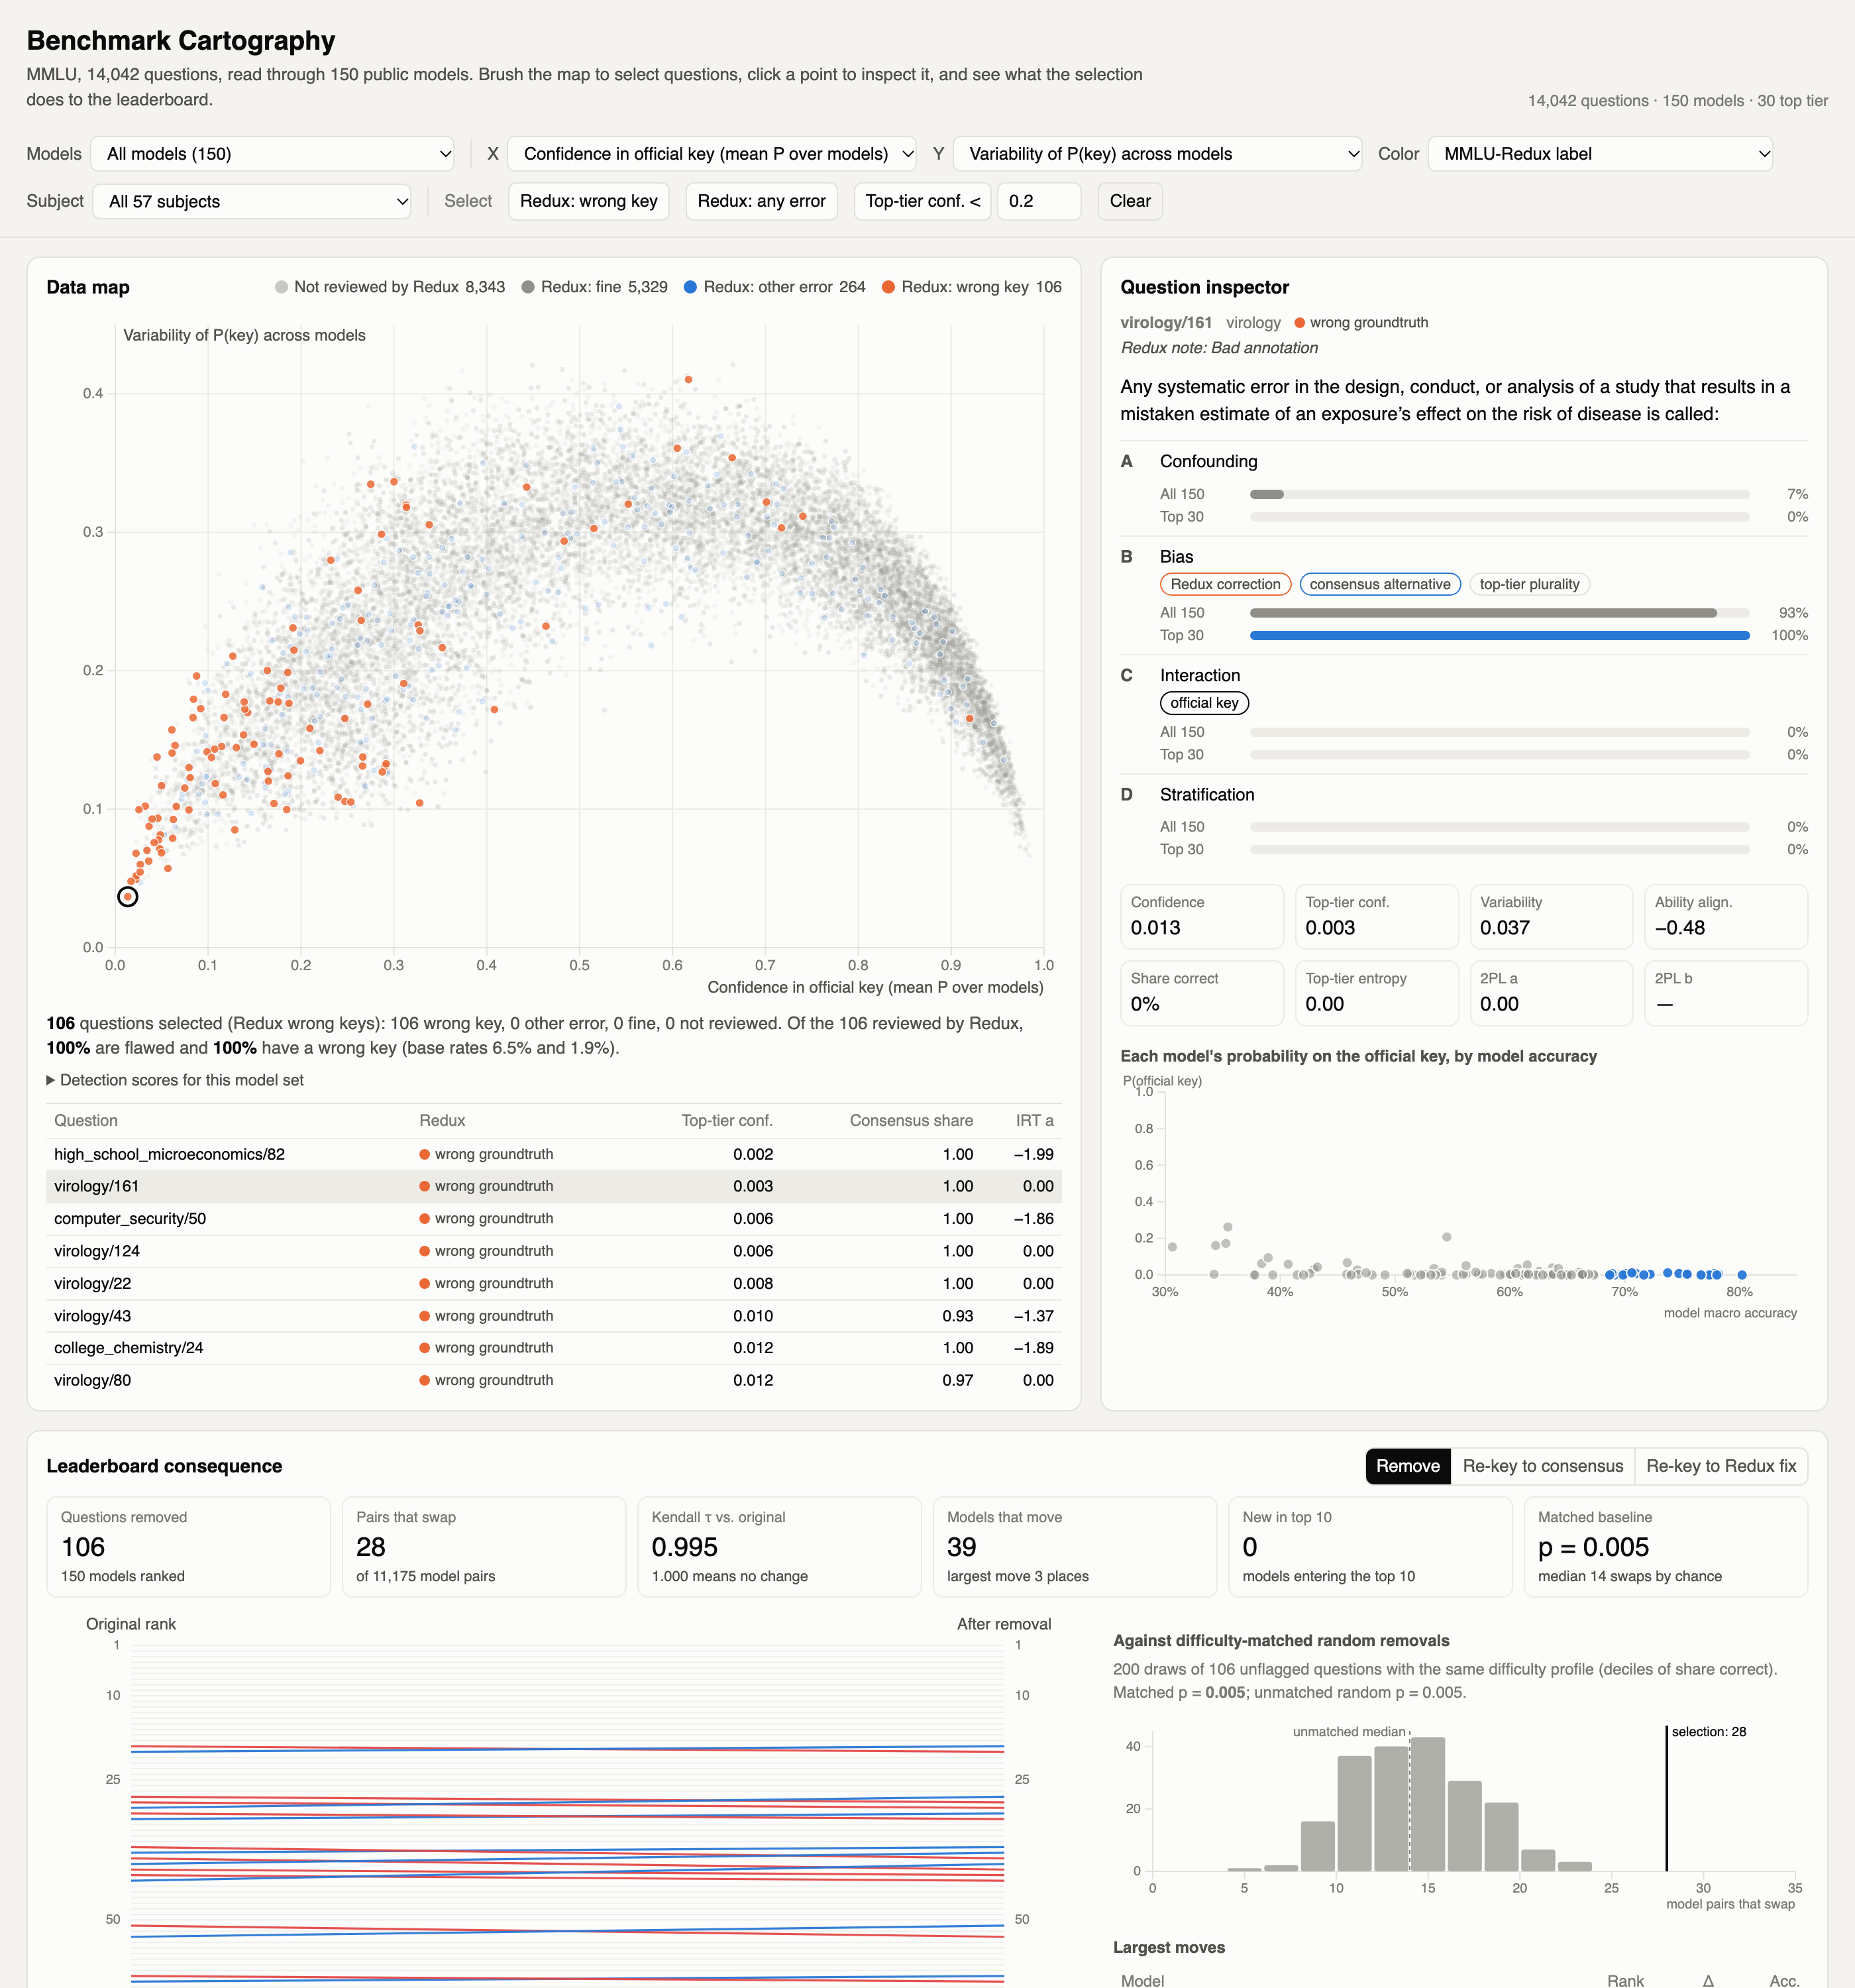
\includegraphics[width=0.95\linewidth]{../report/fig_tool.png}
  \caption{The tool with the 106 known wrong keys selected (orange). Left: the data map. Right: the
  question inspector. Bottom: the leaderboard view.}
\end{figure}

It has three linked views, one for each task an analyst does.

\textbf{View 1: the data map (``where should I look?'').} Every one of the 14,042 questions is a
\textbf{dot}. Left to right is how much models believed the official answer; bottom to top is how
much they disagreed. Dots can be coloured by what the expert checkers found (grey for unchecked,
orange for wrong key). You can drag a box to select a region and change what the axes show. The
orange wrong-key dots pile up in \textbf{one corner}: models agree with each other, but against the
key.

\textbf{View 2: the question inspector (``is this question really broken?'').} Clicking a dot
shows the question and options, the official answer and the answer the top models prefer instead,
\textbf{vote bars} for all 150 models and for the top 30, and a small scatter plot of each model's
belief in the official answer against how good that model is overall. For a fair hard question the
dots \textbf{rise to the right}; for a wrong key they are \textbf{flat at zero or falling}.

\textbf{View 3: the leaderboard consequence (``does it matter?'').} With questions selected, you can
\textbf{remove} them, \textbf{re-key} them to the answer the top models chose, or re-key them to the
experts' correction. The tool \textbf{re-ranks all 150 models in your browser} and shows how many
pairs of models swap places, a \textbf{slope chart} of who moved, and a \textbf{fairness check}: it
removes random questions of the same difficulty 200 times and compares. If your selection causes far
more reshuffling than random questions, the effect is real. This gives a \textbf{p-value}; small
means ``unlikely to be chance''.

\textbf{Extras.} \emph{Model subsets} redo everything using only some models (only ``base'' models,
or one per family), to check the results don't depend on a group of similar models. \emph{Study mode}
(add \texttt{?study} to the link) hides all expert labels so someone can judge questions from model
evidence alone.

\section{What we found}

\subsection*{Finding 1: wrong keys sit in their own corner of the map}
For wrong-key questions the top models put a typical \textbf{12\%} belief on the official answer;
for normal questions, \textbf{82\%}. Other kinds of flaws (such as unclear wording) do \emph{not} form
a clear group: models get confused by them but don't agree on an alternative.

\subsection*{Finding 2: top-tier confidence finds wrong keys well, and modestly beats IRT}
We measured detection with \textbf{AUPRC}, a score where random guessing equals the rate at which the
thing occurs (1.9\% here). Higher is better.

\begin{center}\small
\begin{tabular}{@{}lc@{}}
\toprule
Method & AUPRC \\
\midrule
Random guessing & 0.019 \\
Majority vote of all models & 0.176 \\
IRT difficulty & 0.211 \\
\textbf{Our top-tier confidence} & \textbf{0.355} (about 19$\times$ random) \\
\bottomrule
\end{tabular}
\end{center}

\begin{itemize}
  \item Going down our list of most suspicious questions, \textbf{19 of the first 25} are real wrong keys.
  \item When the top models clearly agree on an alternative, it \textbf{matches the experts'
    correction 87\% of the time}: the tool doesn't just flag errors, it proposes fixes.
  \item \textbf{Honest caveat:} our scores overlap heavily with IRT and the extra benefit is modest.
    Our real advantage is what the tool lets a person \emph{see and do next}.
  \item \textbf{Limitation:} no method here finds ambiguous or unclear questions; only wrong keys.
\end{itemize}

\subsection*{Finding 3: fixing errors changes the leaderboard, but only in the middle}
\begin{itemize}
  \item Removing the 106 known wrong keys makes \textbf{28 pairs} of models swap places.
  \item Random questions of the same difficulty swap only about \textbf{14}: twice as much, and
    very unlikely to be chance ($p = 0.001$).
  \item Correcting the keys instead of removing them swaps \textbf{50 pairs}.
  \item \textbf{But} no model enters or leaves the \textbf{top 10}, and none moves more than a few places.
\end{itemize}
In plain words: the mistakes don't change who is best, but they \textbf{can flip comparisons between
nearly identical models}. Claims like ``our tweaked version beats the original by 0.2\%'' are exactly
what a bad key can get wrong.

\subsection*{Finding 4: new suspected errors nobody had checked}
Among the 8,300 unchecked questions, 289 look strongly suspicious. Two examples:
\begin{itemize}
  \item \textbf{``Which actress played a Vulcan in \emph{Star Trek II}?''} The key says Helen Hunt;
    83\% of top models say \textbf{Kirstie Alley}, who did play the role.
  \item \textbf{``Which is \emph{not} a primary facial expression?''} The key says ``surprise'', but
    surprise \emph{is} a basic expression; 97\% of top models say \textbf{``love''}.
\end{itemize}

\section{How the tool is used: three usage scenarios}

We planned to watch 3 experts use the tool while thinking aloud, but could not recruit anyone during
Thanksgiving week. Instead, as is common in visualization research, we wrote \textbf{usage
scenarios}: step-by-step walkthroughs on real questions.

\begin{figure}[!htb]
  \centering
  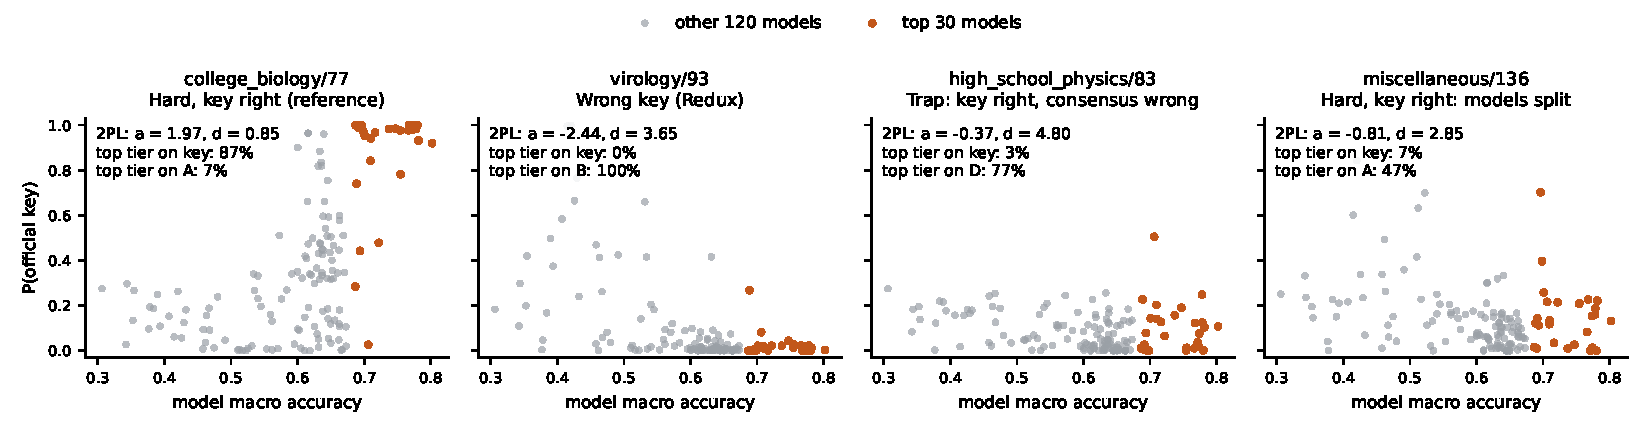
\includegraphics[width=\linewidth]{../report/fig_scenarios.pdf}
  \caption{Each model's belief in the official answer (up) against how good the model is overall
  (right); the 30 strongest models are orange. Left: a fair hard question, where stronger models do
  better. The other three look identical to IRT but differ in how the models vote.}
\end{figure}

\begin{enumerate}
  \item \textbf{Finding errors nobody checked.} Drag a box over the suspicious corner among the grey,
    unchecked dots, click through, and within minutes find the Star Trek and facial-expression
    questions.
  \item \textbf{Wrong key, or just hard?} This is where the tool shows its value. Three questions
    look \textbf{identical to IRT} (very hard, strong models doing worse), yet the tool shows they
    are different:
    \begin{itemize}
      \item \emph{Filovirus shape (virology):} all 30 top models pick the same alternative, so it is a
        \textbf{wrong key}.
      \item \emph{``If Christmas is a Saturday, what day is New Year's?''} The top models split almost
        evenly between two wrong answers. When models \textbf{don't agree on an alternative}, they are
        just failing a hard question; the key (Saturday) is correct.
      \item \emph{Concave mirror (physics):} 77\% of top models agree on an answer, but \textbf{they are
        wrong} and the key is right. Model agreement is \textbf{evidence, not proof}, so the tool
        shows the evidence and leaves the final call to a person.
    \end{itemize}
  \item \textbf{Does it matter?} Select the known wrong keys, remove them, and watch the leaderboard
    reshuffle: the effect beats random, stays in the middle of the table, and shrinks but persists on
    model subsets.
\end{enumerate}

\section{Honest limitations}
\begin{itemize}
  \item Only one benchmark (MMLU) and one testing setup.
  \item The 150 models over-represent small, similar models.
  \item The ``ground truth'' comes from one expert re-check, which is not perfect either.
  \item The method finds wrong keys, \textbf{not} ambiguous questions.
  \item \textbf{No real user study:} the scenarios were done by us, the builders, who already know
    the answers. Running the planned expert study is the main next step.
\end{itemize}

\section{How it all fits together}

\begin{center}\small
\begin{tabularx}{\linewidth}{@{}p{3cm}Yp{2.6cm}@{}}
\toprule
\textbf{Stage} & \textbf{What} & \textbf{Who} \\
\midrule
1. Data & Downloaded 150 models' answers to every question, joined them with the expert labels,
computed the scores and IRT, and saved everything with checksums so others can verify it & Padmapriya \\
2. Analysis & How well the scores detect errors, and how much fixing them moves the leaderboard & Arman \\
3. Tool & The interactive website: map, inspector, leaderboard view & Padmapriya \\
4. Evaluation and delivery & Study protocol, usage scenarios, report, presentation & Both \\
\bottomrule
\end{tabularx}
\end{center}

\textbf{Deliverables.}
\begin{itemize}
  \item The live tool: \url{https://armansam17.github.io/Benchmark-Cartography/}
  \item The 8-page report: \texttt{report/report.pdf}
  \item The code: \url{https://github.com/ArmanSam17/Benchmark-Cartography}, where scripts regenerate
    every number and figure
  \item A presentation with a live demo
\end{itemize}

\end{document}
